\chapter{Specifikacija programske potpore}
		
	\section{Funkcionalni zahtjevi}
			
			\noindent \textbf{Dionici:}
		
		\begin{packed_enum}

		

			\item Naručitelj
			\item Korisnici sustava
					\begin{enumerate}
						\item Organizatori
						\item Posjetitelji
					\end{enumerate}
			\item Administrator			
			\item Razvojni tim
			
		\end{packed_enum}
		
		\noindent \textbf{Aktori i njihovi funkcionalni zahtjevi:}
		
		
		\begin{packed_enum}
			\item  \underbar{Neregistrirani korisnik (inicijator) može:}
			
			\begin{packed_enum}
				
				\item Pregledati najnovije događaje naslovne stranice
				\item registrirati se kao posjetitelj(nema članarine),
				stvoriti novi korisnički račun za koji su mu potrebni korisničko ime, lozinka, ime, prezime i e-mail adresa
				\item registrirati se kao organizator(mjesečna članarina), stvoriti novi korisnički račun za koji su mu potrebni korisničko ime, lozinka, ime, prezime, e-mail adresa
				i broj kreditne kartice
				
				
			\end{packed_enum}
			
			\item  \underbar{Posjetitelj (inicijator) može:}
			
			\begin{packed_enum}
				
				\item pregledavati sva događanja
				\item pregledavati događanja na koje je pretplaćen
				\item izraziti interes s jednom od 3 sljedeće opcije:
				
				\begin{packed_enum}
					\item \textit{sigurno dolazim}
					\item \textit{možda dolazim}
					\item \textit{ne dolazim}
				\end{packed_enum}	
				
				
				\item promijeniti interes 
				\item pregledati recenzije
				\item pisati recenzije za događanja koja su završila u proteklih 48h
				\item brisati recenzije
				\item vidjeti popis aktualnih događanja u odabranom vremenskom razdoblju:
				\begin{packed_enum}
					\item \textit{24h}
					\item \textit{7 dana}
					\item \textit{30 dana}
				\end{packed_enum}
				
				
				\item pretplatiti se na obavijesti o najnovijim događanjima prema zadanim kriterijima:
				
				\begin{packed_enum}
					\item \textit{vrsta događanja}
					\item \textit{područje}
				\end{packed_enum}
				
				\item  na profilu organizatora vidjeti koliki je broj zainteresiranih posjetitelja za pojedini događaj
				
			\end{packed_enum}
			
			\item  \underbar{Organizator (inicijator) može:}
			
			\begin{packed_enum}
				
				\item postavljati najave za događanja koja organiziraju
				\begin{packed_enum}
					\item \textit{koncerti}
					\item \textit{kazališne predstave}
					\item \textit{događanja u klubovima}
					\item \textit{itd.}
				\end{packed_enum}
				\item uređivati i obrisati događaj
				\item unositi podatke, fotografije i videozapise sa događanja kojeg su organizirali
				\item uređivati javni profil
				\item vidjeti kolika je zainteresiranost za pojedini događaj
				\item pregledavati recenzije korisnika
				\item reaktivirati vlastiti profil
				\item dodati način plaćanja članarine
				
			\end{packed_enum}
			
			\item  \underbar{Administrator (inicijator) može:}
			
			\begin{packed_enum}
				
				\item postaviti cijenu članarine
				\item vidjeti popis svih registriranih korisnika i njihovih osobnih podataka
				\item brisati korisnike
				\item brisati recenzije koje su u suprotnosti s pravilima korištenja aplikacije
				\item dodavanje, uređivanje i brisanje kategorije događaja
				
			\end{packed_enum}
			
			
			\item  \underbar{Baza podataka (sudionik) može:}
			
			\begin{packed_enum}
				
				\item pohraniti sve podatke o korisnicima i njihovim ovlastima
				\item pohraniti sve podatke o događanjima
				
				
			\end{packed_enum}
			
		\end{packed_enum}
		
		\eject 
			
			
				
			\subsection{Obrasci uporabe}
				
				
				\subsubsection{Opis obrazaca uporabe}
				
				\noindent \underbar{\textbf{UC1 - Upravljanje korisnicima}}
				\begin{packed_item}
					
					\item \textbf{Glavni sudionik: }Administrator
					\item  \textbf{Cilj:} Pregled registriranih korisnika
					\item  \textbf{Sudionici:} Baza podataka
					\item  \textbf{Preduvjet:} Adiministrator je logiran i korisnik je registriran
					\item  \textbf{Opis osnovnog tijeka:}
					
					\item[] \begin{packed_enum}
						\item Administrator odlazi na svoj profil 
						\item Odabire opciju upravljanja korisnicima
						\item Prikaže se lista registriranih korisnika sa njihovim osobnim podacima
					\end{packed_enum}
					
				\end{packed_item}
				
				\noindent \underbar{\textbf{UC1.1 - Brisanje korisnika}}
				\begin{packed_item}
					
					\item \textbf{Glavni sudionik: }Administrator
					\item  \textbf{Cilj:} Obrisati korisnika i njegovih podataka iz baze
					\item  \textbf{Sudionici:} Baza podataka
					\item  \textbf{Preduvjet:} Administrator je logiran i korisnik postoji u bazi podataka
					\item  \textbf{Opis osnovnog tijeka:}
					
					\item[] \begin{packed_enum}
						\item Administrator odabire opciju pregled korisnika
						\item Odabire opciju brisanje korisnika
					\end{packed_enum}
					
					\item  \textbf{Opis mogućih odstupanja:}
					\item[] \begin{packed_item}
						
						\item[2.a] Korisnik se ne može izbrisati iz baze
						\item[] \begin{packed_enum}
							
							\item Sustav javlja administratoru da ne može izvršiti akciju						
						\end{packed_enum}
						
					\end{packed_item}
					
				\end{packed_item}
				
				\noindent \underbar{\textbf{UC2 - Postavljanje cijena članstva}}
				\begin{packed_item}
					
					\item \textbf{Glavni sudionik: }Administrator
					\item  \textbf{Cilj:} Postavljanje ili promjena cijene članstva
					\item  \textbf{Sudionici:} Baza podataka
					\item  \textbf{Preduvjet:} -
					\item  \textbf{Opis osnovnog tijeka:}
					
					\item[] \begin{packed_enum}
						
						\item Administrator odlazi na svoj profil
						\item Administrator odabire opciju postavljanja cijene članstva i postavlja cijenu
						
					\end{packed_enum}
					
					\item  \textbf{Opis mogućih odstupanja:}
					
					\item[] \begin{packed_item}
						
						\item[2.a] Administrator pokušava postaviti neispravnu cijenu
						\item[] \begin{packed_enum}
							
							\item Akcija se odbija i vraća administratora na početak							
						\end{packed_enum}
						
					\end{packed_item}
					
				\end{packed_item}
				
				\noindent \underbar{\textbf{UC3 - Provjera valjanosti računa}}
				\begin{packed_item}
					
					\item \textbf{Glavni sudionik:}Baza podataka
					\item  \textbf{Cilj:} Provjeriti valjanost računa organizatora
					\item  \textbf{Sudionici:} Baza podataka
					\item  \textbf{Preduvjet:} Organizator koji se želi prijaviti u sustav postoji
					\item  \textbf{Opis osnovnog tijeka:}
					
					\item[] \begin{packed_enum}
						
						\item Prilikom prijave organizatora provjerava se valjanost računa po tome do kada mu je valjana članarina
						\item Provjerom članarine u bazi se postavlja odgovarajuća zastavica vezano za korisnikov račun
					\end{packed_enum}
					
				\end{packed_item}
				
				
				
				\noindent \underbar{\textbf{UC4 - Prijava}}
				\begin{packed_item}
					
					\item \textbf{Glavni sudionik: }Korisnik
					\item  \textbf{Cilj:} Prijava u sustav
					\item  \textbf{Sudionici:} Baza podatka
					\item  \textbf{Preduvjet:} Korisnik je registriran
					\item  \textbf{Opis osnovnog tijeka:}
					
					\item[] \begin{packed_enum}
						
						\item Korisnik unosi sve potrebne podatke u web obrascu i potvrđuje svoj unos
						\item Provjera  ispravnosti unesenih podataka te postoji li korisnik u bazi podataka.
						\item Ako korisnik postoji u bazi podataka, prijavljuje se u sustav i pristupa korisničkim funkcijama
						
					\end{packed_enum}
					
					\item  \textbf{Opis mogućih odstupanja:}
					
					\item[] \begin{packed_item}
						
						\item[2.a] Neispravno korisničko ime/e-mail/lozinka
						\item[] \begin{packed_enum}
							
							\item Sustav obavještava korisnika o neuspjeloj prijavi i vraća ga na stranicu za prijavu
							
						\end{packed_enum}
						
					\end{packed_item}
				\end{packed_item}
				
				\noindent \underbar{\textbf{UC5 - Registracija}}
				\begin{packed_item}
					
					\item \textbf{Glavni sudionik: } Neprijavljeni korisnik
					\item  \textbf{Cilj:}Stvoriti korisnički račun za pristup sustavu
					\item  \textbf{Sudionici:} Baza podataka
					\item  \textbf{Preduvjet:} -
					\item  \textbf{Opis osnovnog tijeka:}
					
					\item[] \begin{packed_enum}
						
						\item Korisnik odabire opciju za registraciju kao posjetitelj ili organizator
						\item Unosi potrebne korisničke podatke
						\item Aplikacija provjerava valjanost unesenih podataka, te provjerava da li korisnik već postoji u bazi podatak
						\item Ako korisnik ne postoji u bazi podataka, aplikacija upisuje u bazu podataka podatke o novom korisniku
					\end{packed_enum}
					
					\item  \textbf{Opis mogućih odstupanja:}
					
					\item[] \begin{packed_item}
						
						\item[3.a] Unos podatka u nedozvoljenom formatu 
						\item[] \begin{packed_enum}
							
							\item Sustav obavještava korisnika o neuspjelom upisu i vraća ga na stranicu za registraciju
							\item Korisnik mijenja potrebne podatke ili odustaje od prijave
							
						\end{packed_enum}
						
						\item[3.b] Odabir zauzetog korisničkog imena ili e-maila
						\item[] \begin{packed_enum}
							
							\item Aplikacija odbija registraciju korisnika i vraća ga na početak registracije
							
						\end{packed_enum}
						
					\end{packed_item}
				\end{packed_item}	
				
				\noindent \underbar{\textbf{UC6 - Pregled najnovijih događaja naslovne stranice}}
				\begin{packed_item}
					
					\item \textbf{Glavni sudionik: } Prijavljeni i neprijavljeni korisnici
					\item  \textbf{Cilj:} Prikazati svima nove događaje
					\item  \textbf{Sudionici:} Baza podataka
					\item  \textbf{Preduvjet:} -
					\item  \textbf{Opis osnovnog tijeka:}
					
					\item[] \begin{packed_enum}
						
						\item Korisniku se prikazuje lista događaja koje može posjetiti
						\item Korisnik odabire događaj i prikazuju se informacije o njemu 
						\item Predstavljanje korisniku  mogućnosti postanka trajnog korisnika stranice nuđenjem mogućnosti prijave kao posjetitelj ili da postane jedan od organizatora
					\end{packed_enum}
					
				\end{packed_item}
				
				\noindent \underbar{\textbf{UC7 - Pregled informacija profila}}
				\begin{packed_item}
					
					\item \textbf{Glavni sudionik: }Korisnik
					\item  \textbf{Cilj:}Pregled informacija profila
					\item  \textbf{Sudionici:} Baza podataka
					\item  \textbf{Preduvjet:} Korisnik je prijavljen u sustav
					\item  \textbf{Opis osnovnog tijeka:}
					
					\item[] \begin{packed_enum}
						
						\item Korisnik odlazi na svoj profil
						\item Ima dostupan pregled svojih informacija
					\end{packed_enum}
				\end{packed_item}
				
				\noindent \underbar{\textbf{UC7.1 - Uređivanje javnog profila}}
				\begin{packed_item}
					
					\item \textbf{Glavni sudionik: } Korisnik
					\item  \textbf{Cilj:} Unos ili izmjena osnovnih podataka
					\item  \textbf{Sudionici:} Baza podataka
					\item  \textbf{Preduvjet:} Korisnik je prijavljen u sustav
					\item  \textbf{Opis osnovnog tijeka:}
					
					\item[] \begin{packed_enum}
						
						\item Korisnik odabire opciju za pregled osnovnih podataka
						\item Korisnik mijenja podatke
						\item Korisnik sprema podatke i baza podataka se ažurira
					\end{packed_enum}
					
					\item  \textbf{Opis mogućih odstupanja:}
					
					\item[] \begin{packed_item}
						
						\item[2.a] Korisnik je promijenio podatke, ali nije odabrao opciju "Spremi promjenu"
						\item[] \begin{packed_enum}
							\item Sustav obavještava korisnika da nije spremio podatke prije izlaska iz prozora 
						\end{packed_enum}
						
						\item[3.a] Korisnik želi spremiti promjenu, ali podaci su promijenjeni u neispravne podatke
						\item[] \begin{packed_enum}
							\item Sustav upozorava korisnika da mora unijeti ispravne podatke kao i kod registracije
						\end{packed_enum}
						
					\end{packed_item}
				\end{packed_item}
				
				\noindent \underbar{\textbf{UC8 - Pregled događaja za koje je korisnik zainteresiran}}
				\begin{packed_item}
					
					\item \textbf{Glavni sudionik: }Posjetitelj
					\item  \textbf{Cilj:} Pregledati sve događaje za koje je posjetitelj izrazio zainteresiranost
					\item  \textbf{Sudionici:} Baza podataka
					\item  \textbf{Preduvjet:} Posjetitelj prijavljen u sustav
					\item  \textbf{Opis osnovnog tijeka:}
					
					\item[] \begin{packed_enum}
						
						\item Korisnik odlazi na svoj profil
						\item Odabire opciju pregled događaja za koje sam izrazio interes
					\end{packed_enum}
				\end{packed_item}
				
				
				
				\noindent \underbar{\textbf{UC8.1 - Promjena interesa}}
				\begin{packed_item}
					
					\item \textbf{Glavni sudionik: }Posjetitelj
					\item  \textbf{Cilj:} Promjena interesa za događaj koji zanima posjetitelja
					\item  \textbf{Sudionici:} Baza podataka
					\item  \textbf{Preduvjet:} Korisnik je prijavljen
					\item  \textbf{Opis osnovnog tijeka:}
					
					\item[] \begin{packed_enum}
						
						\item Korisnik pregledava događaj
						\item Odabire opciju pregled događaja za koje je izrazio interes
						\item Pokraj događaja za koji je izrazio interes u padajućem izborniku odabire interes koji želi
					\end{packed_enum}
				\end{packed_item}
				
				\noindent \underbar{\textbf{UC8.2 - Brisanje interesa}}
				\begin{packed_item}
					
					\item \textbf{Glavni sudionik: }Posjetitelj
					\item  \textbf{Cilj:} Obrisati interes za određeni događaj
					\item  \textbf{Sudionici:} Baza podataka
					\item  \textbf{Preduvjet:} Posjetitelj je prijavljen i već ima izraženu zainteresiranost za događaj
					\item  \textbf{Opis osnovnog tijeka:}
					
					\item[] \begin{packed_enum}
						
						\item Korisnik odlazi na svoj profil
						\item Odabire opciju pregled događaja za koje je izrazio interes
						\item Pored događaja za koji je izrazio interes bira opciju "Obrisi interes"
					\end{packed_enum}
				\end{packed_item}
				
				
				
				
				\noindent \underbar{\textbf{UC9 - Pregled napisanih recenzija}}
				\begin{packed_item}
					
					\item \textbf{Glavni sudionik: }Posjetitelj
					\item  \textbf{Cilj:} Pregled napisanih recenzija
					\item  \textbf{Sudionici:} Baza podataka
					\item  \textbf{Preduvjet:} Korisnik je prijavljen
					\item  \textbf{Opis osnovnog tijeka:}
					
					\item[] \begin{packed_enum}
						
						\item Korisnik odlazi na svoj profil
						\item Odabire opciju napisane recenzije
						\item Prikazuje mu se lista napisanih recenzija
					\end{packed_enum}
					
				\end{packed_item}
				
				\noindent \underbar{\textbf{UC9.1 - Uređivanje recenzije}}
				\begin{packed_item}
					
					\item \textbf{Glavni sudionik: }Posjetitelj
					\item  \textbf{Cilj:} Uređivanje recenzije
					\item  \textbf{Sudionici:} Baza podataka
					\item  \textbf{Preduvjet:} Korisnik je prijavljen i od završetka događaja nije prošlo više od 48 sati
					\item  \textbf{Opis osnovnog tijeka:}
					
					\item[] \begin{packed_enum}
						
						\item Korisnik odlazi na svoj profil i odabire opciju „Napisane recenzije“
						\item Ispisuje mu se lista događaja i recenzije koje su napisane
						\item Korisnik odabire opciju uredi recenziju pokraj recenzije koju želi uredit
						\item Izvršava promjene i sprema recenziju
					\end{packed_enum}
					
					\item  \textbf{Opis mogućih odstupanja:}
					
					\item[] \begin{packed_item}
						
						\item[4.a] Korisnik želi ostaviti prazan obrazac recenzije i kliknuti spremi promijene 
						\item[] \begin{packed_enum}
							\item Sustav odbija ostavljanje praznog obrasca
						\end{packed_enum}
						
						\item[4.b] Korisnik želi izaći, a nije kliknuo spremi  
						\item[] \begin{packed_enum}
							\item Sustav ga upozorava da je napisao recenziju a nije kliknuo „Spremi“
						\end{packed_enum}
						
					\end{packed_item}
				\end{packed_item}
				
				\noindent \underbar{\textbf{UC9.2 - Brisanje recenzije}}
				\begin{packed_item}
					
					\item \textbf{Glavni sudionik: }Posjetitelj
					\item  \textbf{Cilj:} Brisanje recenzije za događaj
					\item  \textbf{Sudionici:} Baza podataka
					\item  \textbf{Preduvjet:} Korisnik je prijavljen i od završetka događaja nije prošlo više od 48 sati
					\item  \textbf{Opis osnovnog tijeka:}
					
					\item[] \begin{packed_enum}
						
						\item Korisnik odlazi na svoj profil
						\item Odabire opciju napisane recenzije
						\item Pored događaja i napisane recenzije odabire opciju brisanje recenzije
					\end{packed_enum}
				\end{packed_item}
				
				\noindent \underbar{\textbf{UC10 - Dodavanje novog događaja}}
				\begin{packed_item}
					
					\item \textbf{Glavni sudionik: }Organizator
					\item  \textbf{Cilj:}Dodavanje novog događaja na listu
					\item  \textbf{Sudionici:} Baza podataka
					\item  \textbf{Preduvjet:} Korisnik je prijavljen
					\item  \textbf{Opis osnovnog tijeka:}
					
					\item[] \begin{packed_enum}
						
						\item Korisnik odlazi na svoj profil i odabire opciju dodavanje događaja
						\item Korisnik unosi sve potrebne informacije za taj događaj i sprema ga
					\end{packed_enum}
					
					\item  \textbf{Opis mogućih odstupanja:}
					
					\item[] \begin{packed_item}
						
						\item[3.a] Korisnik je upisao podatke, ali nije odabrao opciju "Spremi promjenu
						\item[] \begin{packed_enum}
							\item Sustav obavještava korisnika da nije spremio podatke prije izlaska iz prozora
						\end{packed_enum}
						
						\item[3.b] Korisnik nije unio potrebne informacije o događaju
						\item[] \begin{packed_enum}
							\item Sustav obavještava korisnika da određene informacije o događaju moraju biti unesene i vraća ga na obrazac za unos
						\end{packed_enum}
						
					\end{packed_item}
				\end{packed_item}
				
				\noindent \underbar{\textbf{UC11 - Pregled vlastitih događaja}}
				\begin{packed_item}
					
					\item \textbf{Glavni sudionik: }Organizator
					\item  \textbf{Cilj:}Pregled vlastitih oraganiziranih događaja
					\item  \textbf{Sudionici:} Baza podataka
					\item  \textbf{Preduvjet:} Organizator prijavljen u sustav
					\item  \textbf{Opis osnovnog tijeka:}
					
					\item[] \begin{packed_enum}
						
						\item Organizator odabire svoj profil
						\item Bira pregled svih svojih događaja
					\end{packed_enum}
				\end{packed_item}
				
				
				\noindent \underbar{\textbf{UC11.1 - Brisanje događaja}}
				\begin{packed_item}
					
					\item \textbf{Glavni sudionik: }Organizator
					\item  \textbf{Cilj:}Obrisati događaj iz baze podataka te obavijestiti posjetitelje
					\item  \textbf{Sudionici:} Baza podataka
					\item  \textbf{Preduvjet:} Događaj postoji u bazi podataka
					\item  \textbf{Opis osnovnog tijeka:}
					
					\item[] \begin{packed_enum}
						
						\item Organizator odlazi na svoj profil
						\item Odabire opciju pregled događaja
						\item Pored određenog događaja bira opciju brisanje događaja
					\end{packed_enum}
				\end{packed_item}
				
				\noindent \underbar{\textbf{UC11.2 - Pregled zainteresiranih posjetitelja}}
				\begin{packed_item}
					
					\item \textbf{Glavni sudionik: }Organizator
					\item  \textbf{Cilj:} Pregled posjetitelja koji su izrazili zainteresiranost za događaj
					\item  \textbf{Sudionici:} Baza podataka
					\item  \textbf{Preduvjet:} Korisnik je prijavljen i događaj je postavljen
					\item  \textbf{Opis osnovnog tijeka:}
					
					\item[] \begin{packed_enum}
						
						\item Korisnik odlazi na svoj profil
						\item Odabire opciju pregled događaja
						\item Pokraj određenog događaja bira na opciju pregled zainteresiranih posjetitelja
					\end{packed_enum}
				\end{packed_item}
				
				
				
				
				\noindent \underbar{\textbf{UC12 - Pregled načina plaćanja}}
				\begin{packed_item}
					
					\item \textbf{Glavni sudionik: }Organizator
					\item  \textbf{Cilj:} Pregled dosadašnjih načina plaćanja
					\item  \textbf{Sudionici:} Baza podataka
					\item  \textbf{Preduvjet:} Korisnik je prijavljen
					\item  \textbf{Opis osnovnog tijeka:}
					
					\item[] \begin{packed_enum}
						
						\item Korisnik odlazi na svoj profil
						\item Odabire opciju pregled plaćanja
					\end{packed_enum}
				\end{packed_item}			
				
				\noindent \underbar{\textbf{UC12.1 - Dodavanje načina plaćanja}}
				\begin{packed_item}
					
					\item \textbf{Glavni sudionik: }Organizator
					\item  \textbf{Cilj:} Dodati način plaćanja
					\item  \textbf{Sudionici:} Baza podataka
					\item  \textbf{Preduvjet:} Korisnik je prijavljen
					\item  \textbf{Opis osnovnog tijeka:}
					
					\item[] \begin{packed_enum}
						
						\item Korisnik odlazi na svoj profil
						\item Odabire opciju pregled plaćanja
						\item Može dodati karticu ili paypal račun
					\end{packed_enum}
				\end{packed_item}
				
				\noindent \underbar{\textbf{UC12.2 - Brisanje načina plaćanja}}
				\begin{packed_item}
					
					\item \textbf{Glavni sudionik: }Organizator
					\item  \textbf{Cilj:} Obrisati način plaćanja
					\item  \textbf{Sudionici:} Baza podataka
					\item  \textbf{Preduvjet:} Korisnik je prijavljen
					\item  \textbf{Opis osnovnog tijeka:}
					
					\item[] \begin{packed_enum}
						
						\item Korisnik odlazi na svoj profil
						\item Odabire opciju pregled plaćanja
						\item Briše željeni način plaćanja
					\end{packed_enum}
				\end{packed_item}
				
				\noindent \underbar{\textbf{UC13 - Pregled događaja}}
				\begin{packed_item}
					
					\item \textbf{Glavni sudionik: }Posjetitelj
					\item  \textbf{Cilj:} Pregled svih događaja
					\item  \textbf{Sudionici:} Baza podataka
					\item  \textbf{Preduvjet:} Korisnik je prijavljen
					\item  \textbf{Opis osnovnog tijeka:}
					
					\item[] \begin{packed_enum}
						
						\item Korisnik odlazi na naslovnu stranicu
						\item Prikazuje se popis svih događanja
					\end{packed_enum}
				\end{packed_item}
				
				\noindent \underbar{\textbf{UC13.1 - Izražavanje interesa}}
				\begin{packed_item}
					
					\item \textbf{Glavni sudionik: }Posjetitelj
					\item  \textbf{Cilj:} Izražavanje interesa za događaj koji zanima posjetitelja
					\item  \textbf{Sudionici:} Baza podataka
					\item  \textbf{Preduvjet:} Korisnik je prijavljen
					\item  \textbf{Opis osnovnog tijeka:}
					
					\item[] \begin{packed_enum}
						
						\item Korisnik pregledava događaj
						\item Odabire opciju izrazi interes za događaj
						\item Bira željeni interes između ponuđenih
					\end{packed_enum}
				\end{packed_item}
				
				\noindent \underbar{\textbf{UC14 - Pregled svih informacija o događaju}}
				\begin{packed_item}
					
					\item \textbf{Glavni sudionik: }Posjetitelj
					\item  \textbf{Cilj:} Pregledati više informacija o događaju te njegovu zainteresiranosti
					\item  \textbf{Sudionici:} Baza podataka
					\item  \textbf{Preduvjet:} Prijava u sustav kao posjetitelj
					\item  \textbf{Opis osnovnog tijeka:}
					
					\item[] \begin{packed_enum}
						
						\item Korisnik pregledava događaje
						\item Pokraj događaja odabire opciju pregled vise informacija o događaju
					\end{packed_enum}
				\end{packed_item}
				
				\noindent \underbar{\textbf{UC14.1 - Pisanje recenzije}}
				\begin{packed_item}
					
					\item \textbf{Glavni sudionik: }Posjetitelj
					\item  \textbf{Cilj:} Pisanje recenzije nakon završenog događaja
					\item  \textbf{Sudionici:} Baza podataka
					\item  \textbf{Preduvjet:} Posjetitelj je prijavljen i od završetka događaja je prošlo manje od 48 sati
					\item  \textbf{Opis osnovnog tijeka:}
					
					\item[] \begin{packed_enum}
						
						\item Korisnik odabire pregled događaja u proteklih 48 sati na naslovnici
						\item Pored događaja odabire opciju napiši recenziju
						\item Korisnik piše recenziju i sprema ju
					\end{packed_enum}
					
					\item  \textbf{Opis mogućih odstupanja:}
					
					\item[] \begin{packed_item}
						
						\item[2.a] Korisnik želi dodati recenziju za događaj za koji je već napisao recenziju
						\item[] \begin{packed_enum}
							\item Sustav odbija akciju i obavještava ga da je već napisao recenziju za događaj i da može samo nju uredit
						\end{packed_enum} 
						
						\item[3.a] Posjetitelj je napisao  recenziju ali nije odabrao opciju spremi.
						\item[] \begin{packed_enum}
							\item Sustav ga upozorava da je recenzija napisana, ali nije odabrao opciju spremi
						\end{packed_enum}
						
						\item[3.b] Posjetitelj nije ispunio obazac za recenziju, a želi kliknut spremi 
						\item[] \begin{packed_enum}
							\item Sustav odbija dodavanje recenzije i upozorava korisnika da ne može ne napisati ništa
						\end{packed_enum}
					\end{packed_item}
				\end{packed_item}
				
				\noindent \underbar{\textbf{UC15 - Plaćanje članarine}}
				\begin{packed_item}
					
					\item \textbf{Glavni sudionik: }Organizator
					\item  \textbf{Cilj:} Uplata mjesečne članarine
					\item  \textbf{Sudionici:} Baza podataka
					\item  \textbf{Preduvjet:} Korisnik je prijavljen
					\item  \textbf{Opis osnovnog tijeka:}
					
					\item[] \begin{packed_enum}
						
						\item Korisnik odlazi na svoj profil
						\item Odabire opciju plati članarinu
						\item Korisnik odabire opciju plaćanja mjesečne članarine i izvršava akciju
					\end{packed_enum}
					
					\item  \textbf{Opis mogućih odstupanja:}
					
					\item[] \begin{packed_item}
						
						\item[3.a] Transakcija nije uspjela
						\item[] \begin{packed_enum}
							
							\item Sustav javlja korisniku da se uplata nije dogodila i vraća ga na mjesto izvršavanja transakcije
							
						\end{packed_enum}
						
					\end{packed_item}
				\end{packed_item}
				
				\noindent \underbar{\textbf{UC15.1 - Reaktivacija profila}}
				\begin{packed_item}
					
					\item \textbf{Glavni sudionik: } Baza podataka
					\item  \textbf{Cilj:} Ponovna aktivacija organizatorovog profila
					\item  \textbf{Sudionici:} Organizator
					\item  \textbf{Preduvjet:} Organizator je platio članarinu
					\item  \textbf{Opis osnovnog tijeka:}
					
					\item[] \begin{packed_enum}
						
						\item Nakon plaćanja članarine u bazi podataka se bilježi da je članarina plaćena
						\item Organizatoru se omogućuje pristup svim mogućnostima sustava
					\end{packed_enum}
				\end{packed_item}
				
				
				
				\noindent \underbar{\textbf{UC16 - Pregled organizatora}}
				\begin{packed_item}
					
					\item \textbf{Glavni sudionik: }Posjetitelj
					\item  \textbf{Cilj:} Prikaz liste svih organizatora
					\item  \textbf{Sudionici:} Baza podataka
					\item  \textbf{Preduvjet:} Posjetitelj je prijavljen
					\item  \textbf{Opis osnovnog tijeka:}
					
					\item[] \begin{packed_enum}
						
						\item Korisnik odlazi na svoj profil
						\item Odabire opciju pregled svih organizatora
					\end{packed_enum}
				\end{packed_item}
				
				\noindent \underbar{\textbf{UC16.1 - Prikaz profila organizatora}}
				\begin{packed_item}
					
					\item \textbf{Glavni sudionik: }Posjetitelj
					\item  \textbf{Cilj:} Prikaz detalja o profilu organizatora
					\item  \textbf{Sudionici:} Baza podataka
					\item  \textbf{Preduvjet:} Posjetitelj je prijavljen
					\item  \textbf{Opis osnovnog tijeka:}
					
					\item[] \begin{packed_enum}
						\item Korisnik odlazi na svoj profil
						\item Odabire opciju pregled svih organizatora
						\item Pored organizatora bira opciju za prikaz više detalja
					\end{packed_enum}
				\end{packed_item}
				
				\noindent \underbar{\textbf{UC17 - Odabir opcije za slanje automatskih obavijesti o najnovijim događajima}}
				\begin{packed_item}
					
					\item \textbf{Glavni sudionik: }Posjetitelj
					\item  \textbf{Cilj:} Odabir postavki za slanje automatskih obavijesti o najnovijim događanjima
					\item  \textbf{Sudionici:} Baza podataka
					\item  \textbf{Preduvjet:} Korisnik je prijavljen
					\item  \textbf{Opis osnovnog tijeka:}
					
					\item[] \begin{packed_enum}
						\item Korisnik odlazi na svoj profil
						\item Odabire opciju za postavke obavijesti
						\item Odabire kriterije prema kojima će dobivati obavijesti
					\end{packed_enum}
					
					\item  \textbf{Opis mogućih odstupanja:}
					
					\begin{packed_item}
						
						\item[3.a] Korisnik je odabrao postavke, ali nije odabrao opciju "Spremi promjenu"
						\item[] \begin{packed_enum}
							
							\item Sustav obavještava korisnika da nije spremio podatke prije izlaska iz prozora
							
						\end{packed_enum}
					\end{packed_item}
				\end{packed_item}
					
			
				
				
				\subsubsection{Dijagrami obrazaca uporabe}
					
					\begin{figure}[H]
						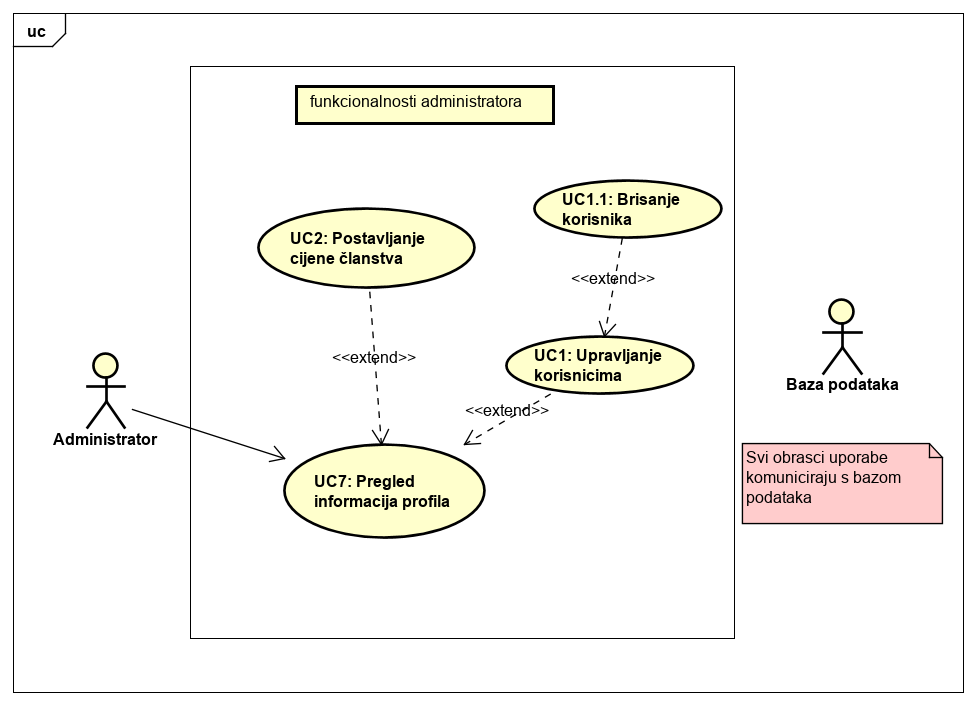
\includegraphics[width=\linewidth]{slike/funkcionalnostiAdministratora.PNG}
						\centering
						\caption{Dijagram obrasca uporabe, funkcionalnosti administratora}
						\label{fig:UCdijagram1}
					\end{figure}
					
					\begin{figure}[H]
						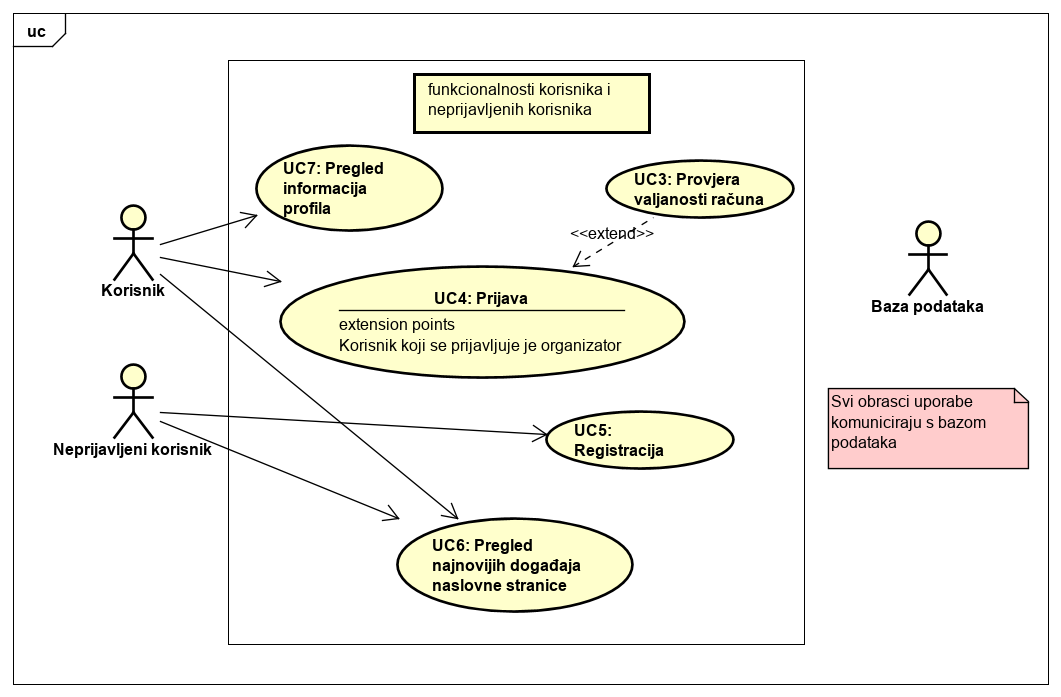
\includegraphics[width=\linewidth]{slike/funkcionalnostSvihKorisnika.PNG}
						\centering
						\caption{Dijagram obrasca uporabe, funkcionalnosti prijavljenih i neprijavljenih korisnika}
						\label{fig:UCdijagram2}
					\end{figure}
					
					\begin{figure}[H]
						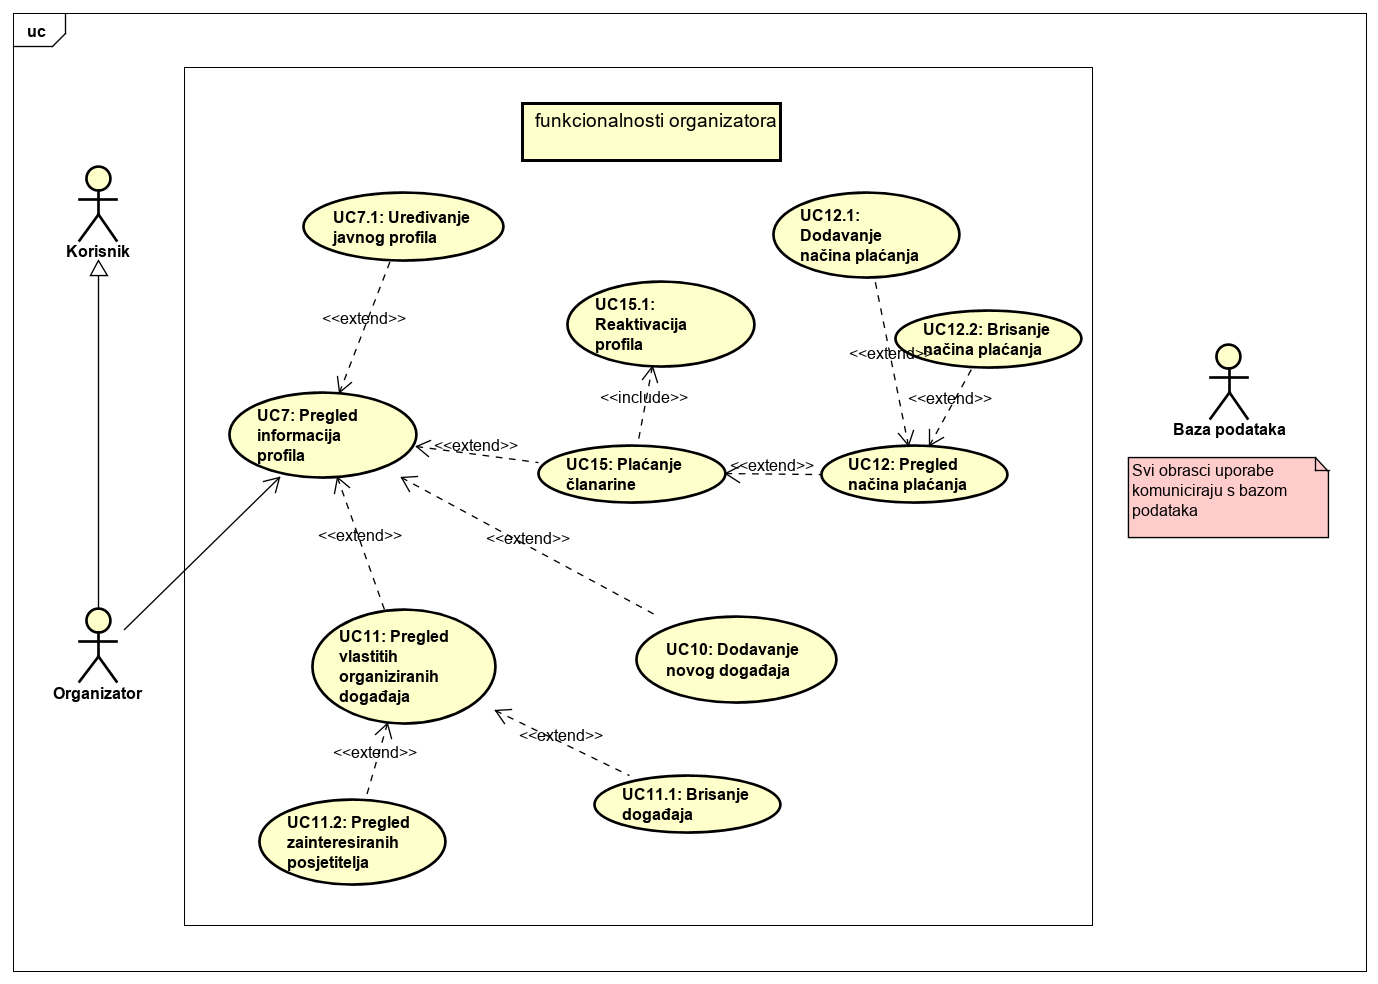
\includegraphics[width=\linewidth]{slike/funkcionalnostiOrganizatora.PNG}
						\centering
						\caption{Dijagram obrasca uporabe, funkcionalnosti organizatora}
						\label{fig:UCdijagram3}
					\end{figure}
					
					\begin{figure}[H]
						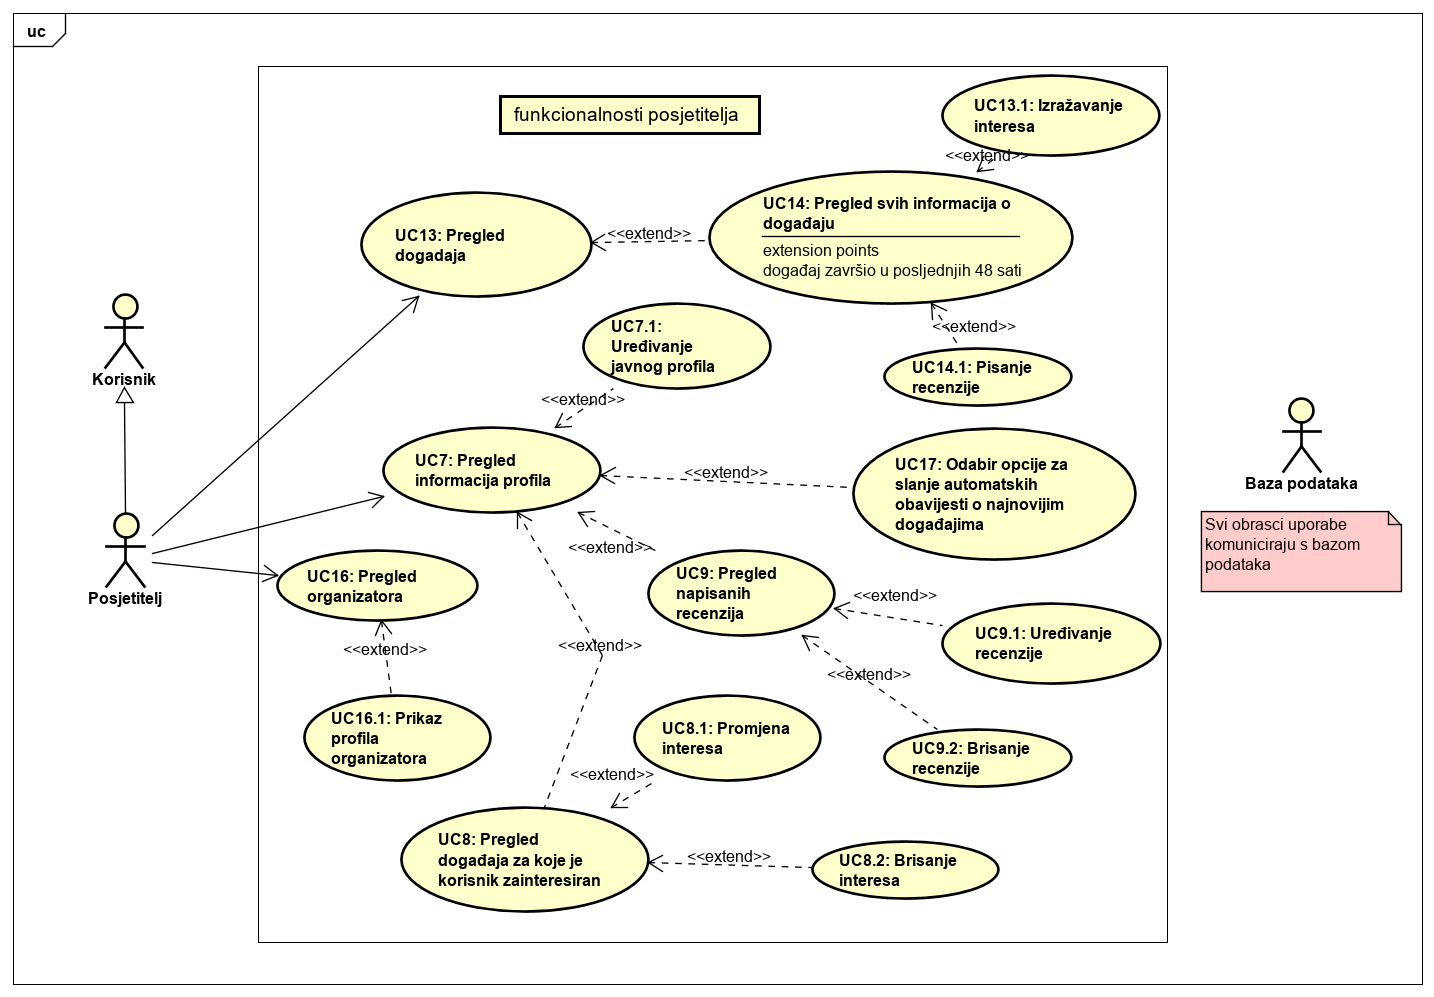
\includegraphics[width=\linewidth]{slike/funkcionalnostiPosjetitelja.PNG}
						\centering
						\caption{Dijagram obrasca uporabe, funkcionalnosti posjetitelja}
						\label{fig:UCdijagram4}
					\end{figure}
				
				
			
				\eject		
				
			\subsection{Sekvencijski dijagrami}
				
				\textbf{Obrazac uporabe UC1 – Pregled informacija profila}\\
				
				\normalfont{Administrator šalje zahtjev za prikaz korisnika. Poslužitelj dohvaća sve korisnike i prikazuje ih. Administrator prolazi kroz sve korisnike, pregledava sve informacije njihovog korisničkog profila i ako želi odaberi opciju brisanje korisnika.}
				
				\normalfont\noindent{Odabiranjem opcije brisanja korisnika šalje zahtjev poslužitelju za brisanje korisničkog profila navedenog korisnika. Poslužitelj zatim šalje zahtjev bazi podataka te uklanja korisnika. Nakon uklanjanja poslužitelj obavještava o obavljenoj operaciji.}
				
				\begin{figure}[H]
					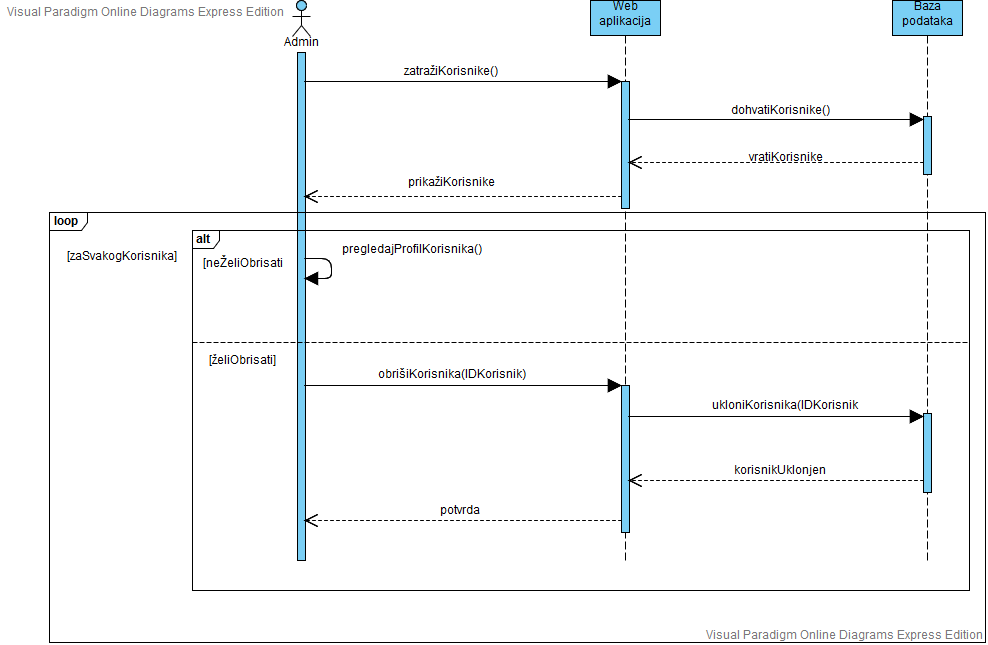
\includegraphics[width=\linewidth]{slike/uc1.PNG}
					\centering
					\caption{Sekvencijski dijagram za UC1}
					\label{fig:uc1}
				\end{figure}
				
				\pagebreak
				
				\textbf{Obrazac uporabe UC5 – Prijava}\\
				
				\normalfont{Korisnik koristi aplikaciju te pregledava najnovije događaje. Zahtjev se šalje poslužitelju koji zatim dohvaća najnovije događaja iz baze podataka s obzirom na lokalno vrijeme upita korisnikovog zahtjeva.}
				
				\normalfont\noindent{Poslužitelj prikazuje događaja te ih po volji korisnik pojedinačno pregledava.}
				
				\normalfont\noindent{Korisnik se može registrirati te u tom slučaju ispunjava svoje podatke te šalje zahtjev poslužitelju koji zatim stvara registraciju novog korisnika u bazi podataka. Ukoliko je korisnik već registriran ispunjava svoje podatke koje zatim poslužitelj prosljeđuje bazi podataka te se tamo vrši provjera njihove točnosti i zatim se vraća potvrda korisniku o uspješnoj ili neuspješnoj prijavi.}
				
				\begin{figure}[H]
					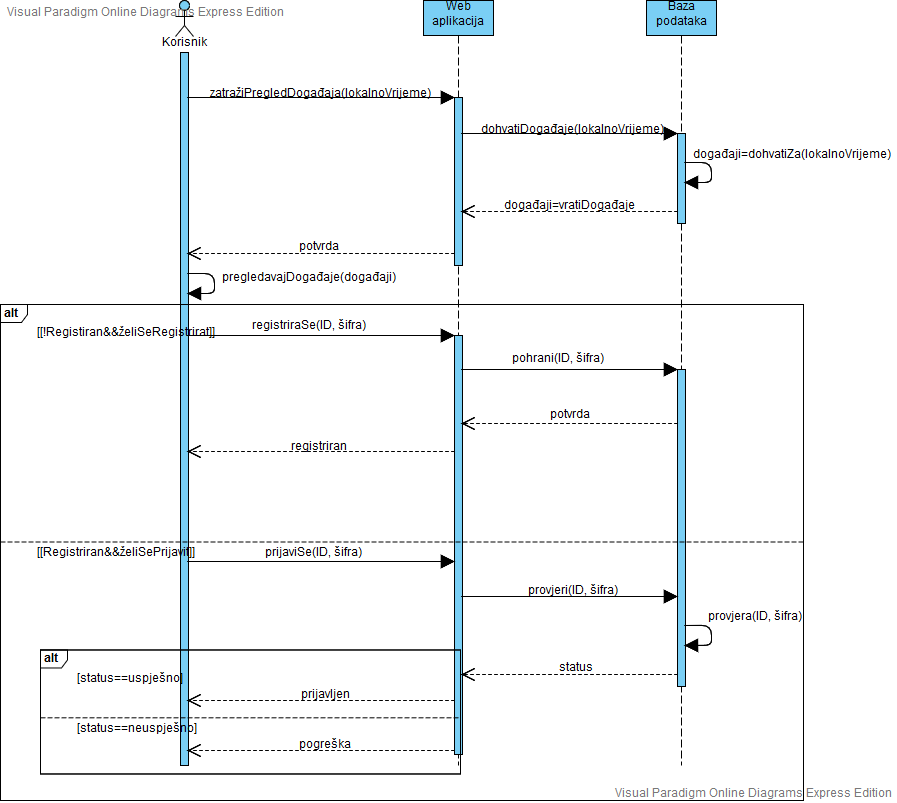
\includegraphics[width=\linewidth]{slike/uc5.PNG}
					\centering
					\caption{Sekvencijski dijagram za UC5}
					\label{fig:uc5}
				\end{figure}
			
				\pagebreak
				
				\textbf{Obrazac uporabe UC10 – Pregled vlastitih organiziranih događaja}\\
				
				\normalfont{Uvjet za korištenje aplikacije kao organizator je plaćanje članarine. U slučaju neplaćene članarine, organizator šalje zahtjeve poslužitelju te odabire opciju plaćanja i ispunjava svoje podatke. Poslužitelj te podatke sprema u bazu podataka te ukoliko je članarina plaćena obavještava organizatora o uspješnoj transakciji.}
				
				\normalfont\noindent{Organizator zatim može pregledavati sve informacije o vlastitim događajima te po izboru ima opcije uređivanja informacija, prikaz svih zainteresiranih korisnika za događaj te brisanje događaja.}
				
				\normalfont\noindent{U slučaju uređivanja informacija i brisanja događa organizator šalje zahtjeve poslužitelju koji te promjene pohranjuje u bazi podataka za navedeni događaj.}
				
				\normalfont\noindent{Ako koristi prikaz svih zainteresiranih korisnika, poslužitelj mu vraća listu svih profila korisnika koji su izrazili interes za događaj iz baze podataka te po izboru pregledava pojedinačni profil.}
				
				\begin{figure}[H]
					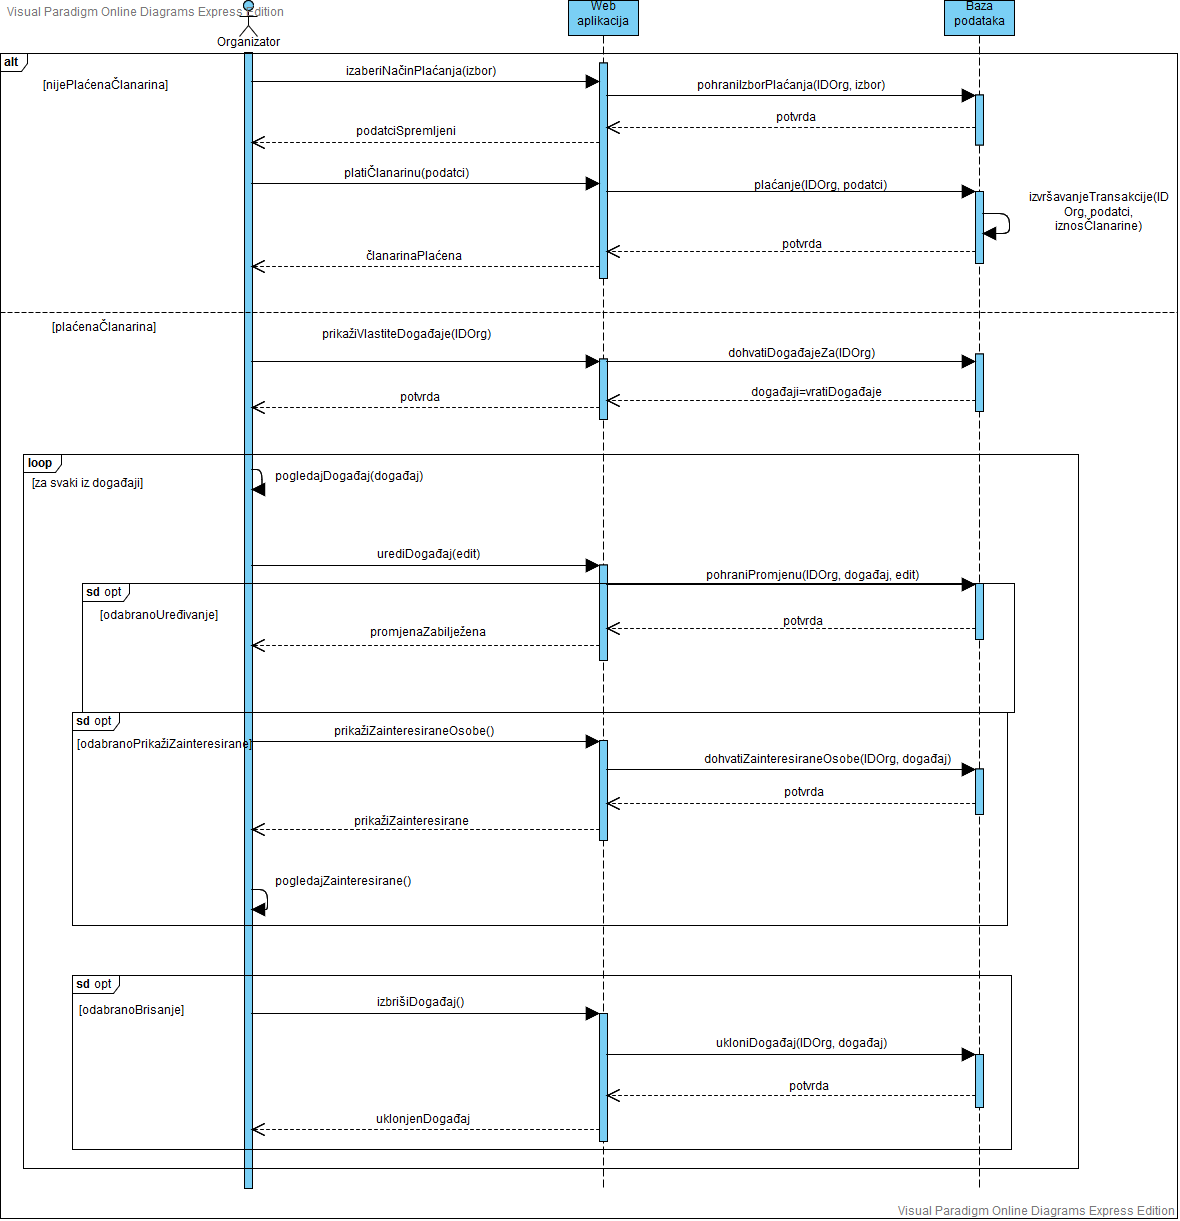
\includegraphics[width=\linewidth]{slike/uc10.PNG}
					\centering
					\caption{Sekvencijski dijagram za UC10}
					\label{fig:uc10}
				\end{figure}
				
				\pagebreak
				
				\textbf{Obrazac uporabe UC13- Pregled događaja prema kriteriju}\\
				
				\normalfont{Posjetitelj unosi kriterije za pregled događaja te šalje zahtjev poslužitelju. Poslužitelj dohvaća događaje sa navedenim kriterijima iz baze podataka te ih prikazuje, inače ako ne postoje javlja grešku posjetitelju. Posjetitelj prolazi kroz svaki događaj i pregledava informacije o svakome. Ako se događaj nije još održao posjetitelj izražava svoj interes te šalje zahtjev poslužitelju. Poslužitelj za navedeni događaj pohranjuje posjetiteljev interes u bazi podataka te ga obavještava da je njegov interes spremljen.}
				
				\normalfont\noindent{Ukoliko se događaj već odvio te je prošlo više od 48 sati od njegovog kraja, posjetitelj može napisati svoju recenziju navedenog događaja te poslati zahtjev poslužitelju. U tom slučaju poslužitelj sprema recenziju događaja posjetitelja u bazi podataka te obavještava posjetitelja da je recenzija spremljena.}
				
				\begin{figure}[H]
					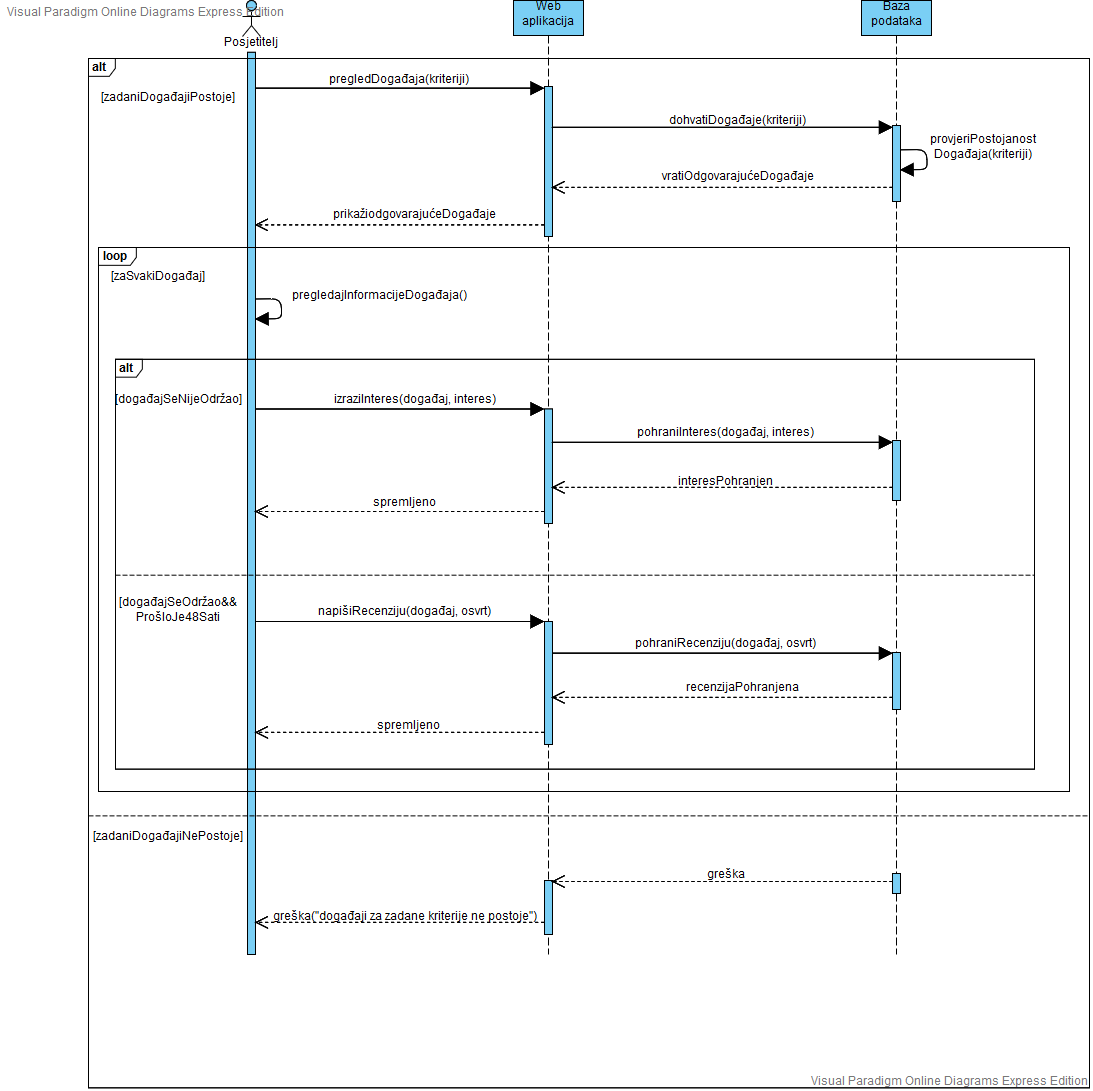
\includegraphics[width=\linewidth]{slike/uc13.PNG}
					\centering
					\caption{Sekvencijski dijagram za UC13}
					\label{fig:uc13}
				\end{figure}
			
				\pagebreak
				
				\eject
	
		\section{Ostali zahtjevi}
		
		\normalfont{
			\begin{packed_item}
				\item \normalfont{Mora biti podržan rad aplikacije ukoliko ga više korisnika koristi istovremeno u stvarnom vremenu}
				\item \normalfont{Moraju biti podržani hrvatski dijakritici}
				\item \normalfont{Izvršavanje učitavanja stranice od slanja zahtjeva sa klijentske strane pa sve do generiranja stranice ne smije trajati dulje od par sekundi}
				\item \normalfont{Korisnički podatci moraju biti zaštićeni od strane drugih korisnika}
				\item \normalfont{Recenzije i događaji moraju se ažurirati kako ih korisnici izmjenjuju/dodaju/brišu}
				\item \normalfont{Osigurati da prije registracije korisnik unese potrebne podatke}
				\item \normalfont{Lozinke se ne spremaju u unesenom obliku, već kriptiranom}
			\end{packed_item}
		}
			 
			 
			 
	